\documentclass[twoside]{book}
\usepackage{makeidx}
\usepackage{fancyhdr}
\usepackage{subfigure}
\usepackage{wrapfig}
\usepackage{amsmath}
\usepackage{latexsym}
\usepackage{graphicx}
\usepackage{amsmath}
\usepackage{alltt}
\usepackage{amssymb}
\usepackage{xspace}
\usepackage{setspace}
%\usepackage[latin1]{inputenc}
\usepackage{moreverb}
\usepackage{multicol}
\usepackage{url}
\usepackage{enumerate}
\usepackage{appendix}
\usepackage{atbegshi}
\usepackage{microtype}
\usepackage[adjust]{cite}
\usepackage{fancyheadings}
%\usepackage[utf8]{inputenc}
%\usepackage{subcaption}
\usepackage{listings}
\usepackage{booktabs}
\usepackage{subfig}

\usepackage[framemethod=TikZ]{mdframed}
%\usepackage{lipsum}
\mdfdefinestyle{MyFrame}{%
    linecolor=blue,
    outerlinewidth=1pt,
    roundcorner=20pt,
    innertopmargin=\baselineskip,
    innerbottommargin=\baselineskip,
    innerrightmargin=20pt,
    innerleftmargin=20pt,
    backgroundcolor=white}
    %backgroundcolor=gray!50!white}
    


\newcommand\myworries[1]{\textcolor{red}{#1}}


\newtheorem{mydef}{Definition}

\newtheorem{
}{Notation}

\usepackage{algpseudocode}
\usepackage{algorithm}
\usepackage{appendix}



\usepackage[pages=some]{background}
\usetikzlibrary{calc}

\usepackage{geometry}


%formato A5
%paperwidth=150mm, 
%paperheight=230mm,

 %formato stampa il mio libro
\geometry{
paperwidth=145mm,
paperheight=225mm,
left=18mm,
right=12mm,
top=8mm,
bottom=12mm,
includehead=true,
includefoot=true,
twoside=true}

%
%\usepackage[cam,a4,center,pdftex]{crop}



\usepackage[pdftex, pdfborder= 0 0 0, citecolor=black, urlcolor=black, linkcolor=black, colorlinks=true, bookmarksopen=false]{hyperref}
\usepackage{bookmark}


    
\newfloat{eqfloat}{h}{eqflts}
\floatname{eqfloat}{Equation}
\makeatletter
\let\c@eqfloat\c@equation
\makeatother

%

\usepackage{listings}
\usepackage{color} %red, green, blue, yellow, cyan, magenta, black, white
\definecolor{mygreen}{RGB}{28,172,0} % color values Red, Green, Blue
\definecolor{mylilas}{RGB}{170,55,241}
\begin{document}


\lstset{language=Matlab,%
    %basicstyle=\color{red},
    breaklines=true,%
    morekeywords={matlab2tikz},
    keywordstyle=\color{blue},%
    morekeywords=[2]{1}, keywordstyle=[2]{\color{black}},
    identifierstyle=\color{black},%
    stringstyle=\color{mylilas},
    commentstyle=\color{mygreen},%
    showstringspaces=false,%without this there will be a symbol in the places where there is a space
    numbers=left,%
    numberstyle={\tiny \color{black}},% size of the numbers
    numbersep=9pt, % this defines how far the numbers are from the text
    emph=[1]{for,end,break},emphstyle=[1]\color{red}, %some words to emphasise
    %emph=[2]{word1,word2}, emphstyle=[2]{style},    
}


%\crop[cam]
%
\author{Matteo Manca}
\title{Neural Networks}




%
%\makeatletter
%\hypersetup{
%pdftitle=\@title, 
%pdfauthor=\@author, 
%pdfsubject={Human Computer Interaction},
%pdfkeywords={Gesture} {Cooperation} {Natural} {Interaction} {Multitouch} {Tangible} {Embodied}}
%
%\makeatother
%
\pagestyle{fancyplain}
\renewcommand{\chaptermark}[1]{\markboth{#1}{}}
\lfoot
[\hrule \vspace{4pt} \footnotesize{Matteo Manca\hfill \textit{Neural Netorks}}]
{\hrule \vspace{4pt} \footnotesize{Matteo Manca\hfill \textit{Neural Netorks}}}
\cfoot{}       
\rfoot[]{}
%
\lhead[\footnotesize{\thepage}]{\footnotesize{\leftmark}}
\chead[]{}          
\rhead[\footnotesize{\leftmark}]{\footnotesize{\thepage}}




\newcommand{\superscript}[1]{\ensuremath{^{\textrm{#1}}}}
\newcommand{\st}[0]{\superscript{st}}
\newcommand{\halfcol}{width=.45\textwidth}
\newcommand{\fullcol}{width=.90\textwidth}
\newcommand{\smallcol}{width=.65\textwidth}
\newcommand{\HRule}{\rule{\linewidth}{0.5mm}}

% create a shortcut to typeset table headings
\newcommand\tabhead[1]{\small\textbf{#1}}
%
\frontmatter
\setlength{\parindent}{15pt}
\setlength{\parskip}{1.2ex plus 0.5ex minus 0.2ex}

\SetBgOpacity{1}
\SetBgScale{1}
\SetBgAngle{0}
\SetBgColor{white}

\newcommand{\BgFingerprint}[2]{
\SetBgContents{
\begin{tikzpicture}[remember picture,overlay]
% draw image

%finger in titles
\node[inner sep=0,opacity=0.12] at  ($ (current page.center) + (0cm,0cm) $)
{\includegraphics[width=20cm]{figures/cover/fingerprint_high}};

%finger in page number
%\node[inner sep=0,opacity=0.12] at  ($ (current page.north east) + (1.65cm,2.3cm) $)
%{\includegraphics[width=1cm]{figures/cover/fingerprint}};

%\node (rect) at  ($ (current page.center) + (3.3cm,6.5cm) $)
 %[draw,opacity=0.9,color=black,fill=white,minimum width=9cm,minimum height=3cm,rounded corners=1cm] {\large #1};

%\node (rect) at  ($ (current page.center) + (3.3cm,4.5cm) $)
 %[draw,opacity=0.9,color=white,fill=white,minimum width=9cm,minimum height=3cm,rounded corners=1cm] {\large  #2};

\end{tikzpicture}
}
}


\begin{center}
{\large \textbf{ Neural Networks\\ 
\vspace{0.2in}Matteo Manca\\ }}
{\small \tt matteomanca@gmail.com}
\end{center}
\vspace{0.2in}

\newsavebox\IBoxA \newsavebox\IBoxB \newlength\IHeight
\newcommand\TwoFig[5]{% Image1 Caption1 Label1 Image2 ...
  \sbox\IBoxA{\includegraphics[width=0.5\textwidth]{#1}}
  \sbox\IBoxB{\includegraphics[width=0.5\textwidth]{#3}}%
  \ifdim\ht\IBoxA>\ht\IBoxB
    \setlength\IHeight{\ht\IBoxB}\else\setlength\IHeight{\ht\IBoxA}\fi%
  \begin{figure}[htb]
\centering
\subfigure[]{%
\includegraphics[height=\IHeight]{#1}
\label{#2}}
\subfigure[]{%
\includegraphics[height=\IHeight]{#3}
\label{#4}}
\caption{#5}
\end{figure}
}


%\input{0.0.notes}
%\input{0.0.titlepage-ita}
%\input{0.0.titlepage-eng}
%\input{Chapters/0_Acknowledgements}
%\input{Chapters/0_abstract}
\cleardoublepage
%
\pagestyle{empty}
\setcounter{tocdepth}{2} %%to decide the deep of the table of content
\setlength{\parskip}{2pt}
\tableofcontents
%\section{section}
%\subsection{subsection}
%\listoffigures
\setlength{\parskip}{1.2ex plus 0.5ex minus 0.2ex}
%
\mainmatter 
\pagestyle{fancyplain}
\renewcommand{\chaptermark}[1]{\markboth{#1}{}}
\lfoot
[\hrule \vspace{4pt} \footnotesize{Matteo Manca\hfill \textit{Neural Netorks}}]
{\hrule \vspace{4pt} \footnotesize{Matteo Manca\hfill \textit{Neural Netorks}}}
\cfoot{}       
\rfoot[]{}
%
\lhead[\footnotesize{\thepage}]{\footnotesize{\leftmark}}
\chead[]{}          
\rhead[\footnotesize{\leftmark}]{\footnotesize{\thepage}}

% paragraph spacing and indentation rules for mainmatter
%
\cleardoublepage

\begin{quotation}
\begin{itshape}
The following notes represent a personal interpretation of the Neural Networks classes of the Coursera machine learning course (https://www.coursera.org/learn/machine-learning/) presented by Professor Andrew Ng . 
\end{itshape}
\end{quotation}

\newpage

\section{Artificial Neural Networks} % Introduction
\label{ANN}

Neural Network is a learning algorithm based on how human brain works and it is very useful to approach different machine learning problems.
In order to better understand why we need another learning algorithm although we already study linear regression and logistic regression, let's see a an example of machine learning problem where ne need complex non-linear hypotheses.


\begin{figure}[H]
\begin{center}
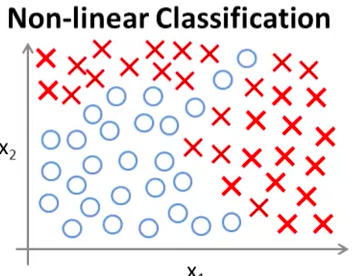
\includegraphics[scale=0.35]{images/non-linear-class}
%[scale=0.45,natwidth=1052, natheight=926]{tbus_acc_30_05.png}
\end{center}
\caption{Example of a non-linear classification problem} 
\label{nn-linear-class}
\end{figure}


If we want to apply logistic regression to this problem we have to use a lot of non linear features like in equation \ref{eq:sigmoidmanyterms} {\bf sigmoid function} (see logistic regression for more explanations about that):


\begin{eqfloat}[H]
\begin{equation}
	g(\Theta_0 + \Theta_1x_1 +  \Theta_2x_2 + \Theta_3x_1x_2 +  \Theta_4x_1^2x_2 + \dots )
\end{equation}
      \addtocounter{equation}{-1}
        \caption{ Sigmoid function with many terms}
        \label{eq:sigmoidmanyterms}
    \end{eqfloat}


So, to get a good classification we need to include a high number of polynomial terms. Logistic regression method works well when we have only two input features, $x_1$ and $x_2$ because in that case we can add all polynomial terms of $x_1$ and $x_2$. In many machine learning problems we will have a lot more feature than just two.

Let's think at the price house prediction problem we saw in previous lectures and suppose to have a classification problem rather than a regression problem. For instance we can imagine to have different features of a house and we want to predict what are the odds that the house will be hold within the next six months:
\\ 
$x_1$ = size \\
$x_2$ = \# bedrooms \\
\vdots \\
$x_{100}$ = \dots \\

In a problem like that reported above, with $n=100$ features, if we want to include the polynomial terms there would be a very huge number of terms. For instance, if we think to include even just the quadratic terms (second order terms, that are the terms obtained as the product of two of these terms - for instance $x_1x_2$ ) in a problem with $n=100$ we obtain about $5000$ features.\\
Asymptotically the number of quadratic terms grows as order of $O(n^2)$, and it is closer to $n^2/2$, in fact $100^2/2 = 5000$.

We demonstrated that also considering just the quadratic terms the number of features is very high, consequently there is a high risk of {\bf overfitting} (see previous lectures for the overfitting problem) the training set and the computation would be too much expensive.
One idea to avoid this high number of features could be to consider just a subset of the terms, for instance $x_1^2, x_2^2, \hdots , x_{100}^2$. In this way the number of features would be smaller but these features would not be enough to represent the dataset represented in figure ~\ref{nn-linear-class}.
In fact if we include only the quadratic features with the original features $x_1, x_2, \hdots, x_n$ we can obtain just lines of the ellipse (Figure \ref{ellipse}) but we cannot fit more complex datasets.

\begin{figure}[H]
\begin{center}
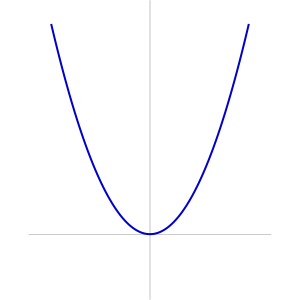
\includegraphics[scale=0.15]{images/ellipse}
%[scale=0.45,natwidth=1052, natheight=926]{tbus_acc_30_05.png}
\end{center}
\caption{Example of a quadratic function} 
\label{ellipse}
\end{figure}

If we think to include the third order (or even higher) polynomial terms the number of features will increase again so we are going to face the same problem described above. Let's see an example to better understand how the number of features $n$ can be very high.
\\
Consider an example of computer vision problem where we want to train a classifier able to examine an image and tell us if the image is a car or not (Remember that an image is a matrix of pixels intensity values).
In our example we have a labeled training set with few label example of cars and a few label of other objects (not cars) , see figure ~\ref{cv-dataset}.

\begin{figure}[H]
\begin{center}
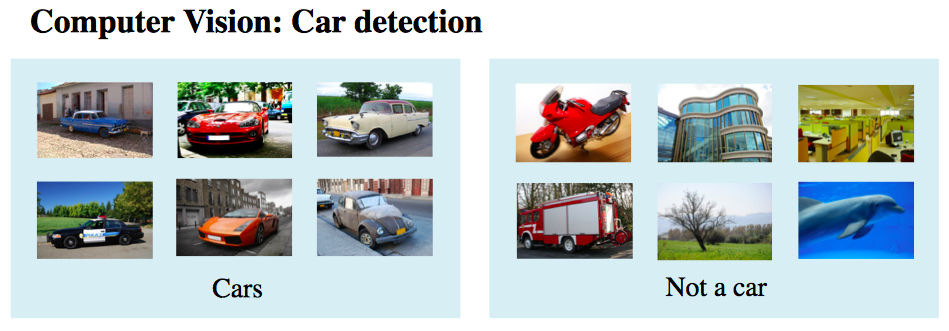
\includegraphics[scale=0.25,natwidth=1357, natheight=2496]{images/cv-dataset}
%[scale=0.45,natwidth=1052, natheight=926]{tbus_acc_30_05.png}
\end{center}
\caption{Computer Vision example dataset} 
\label{cv-dataset}
\end{figure}

We can imagine to plot a object of the dataset. Let's pick a couple of pixel locations (pixel 1 and pixel 2) in our image and plot the object depending on the intensity of pixel 1 and pixel 2 (see figure ~\ref{plotcvproblem})

\begin{figure}[H]
\begin{center}
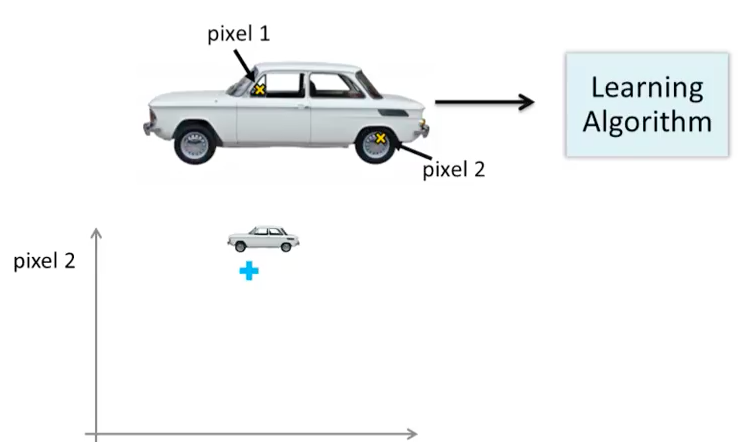
\includegraphics[scale=0.25]{images/plotcvproblem}
%[scale=0.45,natwidth=1052, natheight=926]{tbus_acc_30_05.png}
\end{center}
\caption{Objects plot} 
\label{plotcvproblem}
\end{figure}

Plotting all objects of the dataset we can notice that cars and not-cars end up lying in different regions of the plot (see figure \ref{platoonobjs}) so we need a non-linear hypothesis to try to separate the two classes \{cars, not-cars\}.

\begin{figure}[H]
\begin{center}
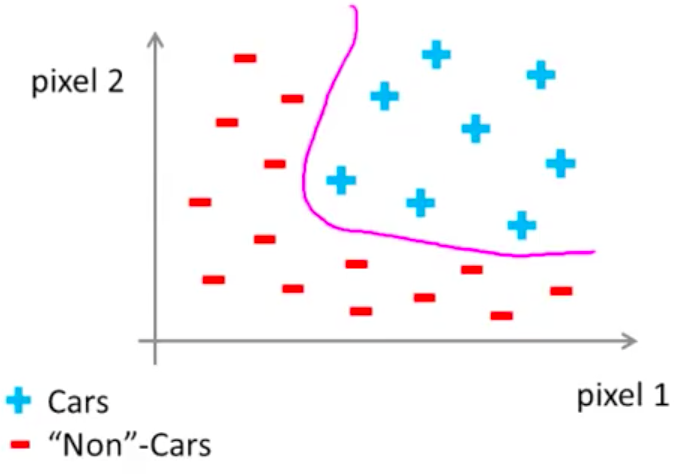
\includegraphics[scale=0.25]{images/platoonobjs}
%[scale=0.45,natwidth=1052, natheight=926]{tbus_acc_30_05.png}
\end{center}
\caption{Plot with all objects of the dataset} 
\label{platoonobjs}
\end{figure}

in the above example we consider just two pixel, but if we use a $50 \times 50$ pixel image the dimension of the features space is $n = 50*50 = 2500$, so we have a vector of $2500$ pixel intensities. If we try to learn a non-linear hypothesis by including all the quadratic terms, we obtain about $3$ million features and it would be too large.

So,we demonstrated that logistic regression with the addition of quadratic (or cubic) features is not a good idea to learn a complex non-linear hypothesis when $n$ is large because we end up with too many features.


\subsection{Model Representation}
Neural networks were developed simulating neurons or network of neurons in the human brain. Let's look how a single neuron looks like:

\begin{figure}[H]
\begin{center}
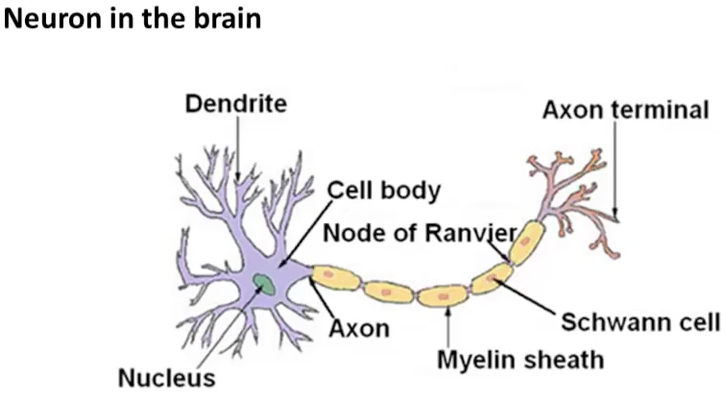
\includegraphics[scale=0.25]{images/neuron}
\end{center}
\caption{A single neuron} 
\label{neuron}
\end{figure}


Neurons are cells in the brain; some things to draw attention to are the {\bf Cell body}, a number of input wires called {\bf dendrites} and a number of output wires called {\bf axons}. We can think to a neuron as a computational unit that receives inputs through dendrites, does some computations and sends an output signal via its axons to other nodes. Neurons comunicate by means of little pulse of electricity 


\subsubsection{Neural Model: Logistic Unit}
In an {Artificial Neural Network} implemented in a computer, we use a very simple model of what a neuron does. We are going to model a neuron as a simple logistic unit (figure \ref{logisticunit}):



\begin{figure}[H]
\begin{center}
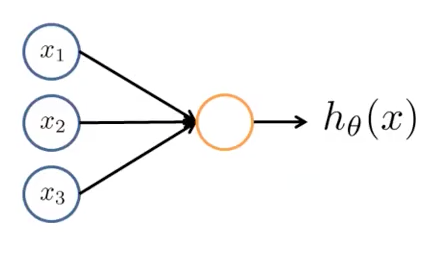
\includegraphics[scale=0.25]{images/logisticunit.png}
\end{center}
\caption{A simple logistic unit} 
\label{logisticunit}
\end{figure}

where $h_{\theta(x)}$ represent the computation of:


\begin{eqfloat}[H]
\begin{equation}
	h_{\theta(x)} = \frac{1}{1 + e^{-\theta x}}
\end{equation}
      \addtocounter{equation}{-1}
        \caption{ Sigmoid function}
        \label{eq:sigmoid}
    \end{eqfloat}




and $\theta$ and $x$ are the parameter vectors:
\begin{equation}
\theta &= \begin{bmatrix}
           \theta_{0} \\
           \theta_{1} \\
           \theta_{2} \\
	     \theta_{3} 
         \end{bmatrix}
          x &= \begin{bmatrix}
           x_{0} \\
           x_{1} \\
           x_{2} \\
	   x_{3} 
         \end{bmatrix}
\end{equation}
         
 Note that we add $x_0$ that is the {\bf bias unit} and we set $x_0 = 1$.  \\
 In neural networks the sigmoid function ( or logistic function) is also called {\bf Activation function} and the parameters $\theta$ are called {\bf weights} of the model. Till now we see just a single neuron, but a neural network is a proof of {\it different neurons models that interact each other }.
 
 
\begin{figure}[H]
\begin{center}
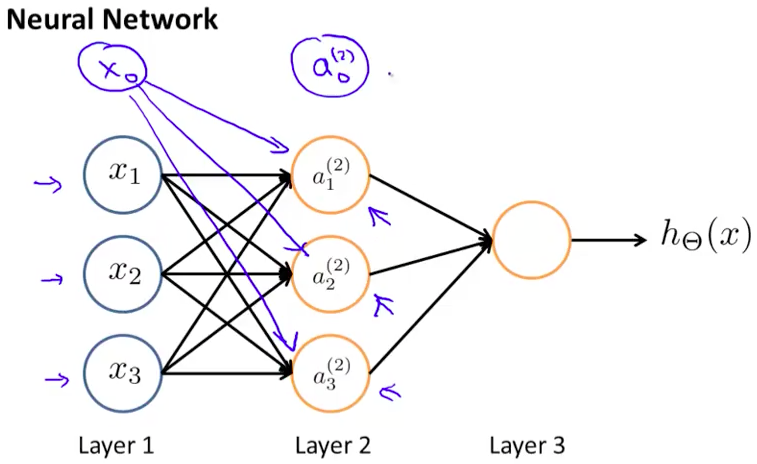
\includegraphics[scale=0.25]{images/neurnet}
\end{center}
\caption{An example of neural network} 
\label{fig:neurnet}
\end{figure}

In figure \ref{fig:neurnet} we have a neural network composed by three neurons $a_1^{2}$, $a_2^{2}$, $a_3^{2}$  more the bias unit $a_0^{2}$; moreover in the above neural network we have multiple layers:

\begin{itemize}
\item {\bf input layer} (layer 1): in this layer we input the features $x_1$, $x_2$ and $x_3$ (of our training set);
\item {\bf hidden layer} (layer 2): it contains values that we don't observe in the training set;
\item {\bf final layer} (layer 3): it has a neuron / units (it can have more units) that output the final value computed by the hypothesis.
\end{itemize}

In order to explain a specific computation of a neural network, in the following we report a some definitions:
\begin{itemize}
\item {\bf $a_i^{(j)}$} : {\bf Activation} of unit $i$ in layer $j$ (i.e., the value that is computed by and that is the output of a specify unit);
\item {\bf $\Theta^{(j)}$}: {\bf matrix of weights} that controls the function mapping from layer $j$ to layer $j+1$.
\end{itemize}

The computation of the diagram in figure ~\ref{fig:neurnet} is reported in equation ~\ref{eq:neurnetcomput}.


\begin{eqfloat}[H]
\begin{equation}
	\begin{aligned}
	a_1^{(2)}  = g(\Theta_{10}^{(1)}x_0 + \Theta_{11}^{(1)}x_1 +  \Theta_{12}^{(1)}x_2 + \Theta_{13}^{(1)}x_3 )\\
	a_2^{(2)}  = g(\Theta_{20}^{(1)}x_0 + \Theta_{21}^{(1)}x_1 +  \Theta_{22}^{(1)}x_2 + \Theta_{23}^{(1)}x_3 )\\
	a_3^{(2)}  = g(\Theta_{30}^{(1)}x_0 + \Theta_{31}^{(1)}x_1 +  \Theta_{32}^{(1)}x_2 + \Theta_{33}^{(1)}x_3 )\\
	h_{\Theta}(x)  =  a_1^{(3)} =  g(\Theta_{10}^{(2)}a_0^{(2)} + \Theta_{11}^{(2)}a_1^{(2)} +  \Theta_{12}^{(2)}a_2^{(2)}+ \Theta_{13}^{(2)}x_3^{(2)} )\\
	\end{aligned}	
\end{equation}
      \addtocounter{equation}{-1}
        \caption{ Neural Network computation}
        \label{eq:neurnetcomput}
    \end{eqfloat}


Summarizing, in our neural network (figure ~\ref{fig:neurnet}) we have:

\begin{itemize}
\item 3 input units (without consider the bias unit);
\item 3 hidden units (without consider the bias unit);
\end{itemize}

$\Theta^{(1)}$ is $3 \times 4$ matrix, so $\Theta^{(1)} \in \mathbb{R}^{3\times4}$.

\begin{mydef}
If a network has $S_j$ units in layer $j$, $S_{j+1}$ units in layer $j+1$, then $\Theta^{(j)}$ is a $S_{j+1} \times S_{j} + 1$ matrix:
\begin{equation}\label{eq:thetadimension}
\Theta^{(j) } \in \mathbb{R}^{S_{j+1} \times S_{j} + 1
\end{equation}
\end{mydef}


\subsection{Feedforward propagation} % Introduction
\label{feedforwardprop}


In this section we'll see how to carry out the computation of the neural network (in figure ~\ref{neurnet1}) efficiently using a {\bf vectorized implementation} and how a neural network can help to learn complex non-linear hypotheses.



\begin{figure}[H]
\begin{center}
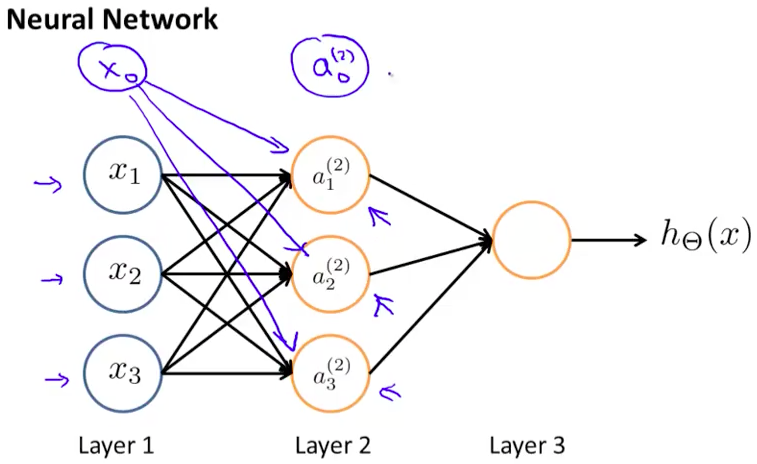
\includegraphics[scale=0.25]{images/neurnet}
\end{center}
\caption{An example of neural network} 
\label{neurnet1}
\end{figure}

\begin{eqfloat}[H]
\begin{equation}
	\begin{aligned}
	a_1^{(2)}  = g(\Theta_{10}^{(1)}x_0 + \Theta_{11}^{(1)}x_1 +  \Theta_{12}^{(1)}x_2 + \Theta_{13}^{(1)}x_3 )\\
	a_2^{(2)}  = g(\Theta_{20}^{(1)}x_0 + \Theta_{21}^{(1)}x_1 +  \Theta_{22}^{(1)}x_2 + \Theta_{23}^{(1)}x_3 )\\
	a_3^{(2)}  = g(\Theta_{30}^{(1)}x_0 + \Theta_{31}^{(1)}x_1 +  \Theta_{32}^{(1)}x_2 + \Theta_{33}^{(1)}x_3 )\\
	h_{\Theta}(x)  =  a_1^{(3)} =  g(\Theta_{10}^{(2)}a_0^{(2)} + \Theta_{11}^{(2)}a_1^{(2)} +  \Theta_{12}^{(2)}a_2^{(2)}+ \Theta_{13}^{(2)}x_3^{(2)} )\\
	\end{aligned}	
\end{equation}
      \addtocounter{equation}{-1}
        \caption{ Neural Network computation}
        \label{eq:neurnetcomput1}
    \end{eqfloat}

Starting from equation \ref{eq:neurnetcomput1} we define some new notation:

\begin{equation}\label{eq:feeddefinitions}
\begin{aligned}
a_1^{(2)}  = g(z_1^{(2)}) \implies z_1^{(2)} = \Theta_{10}^{(1)}x_0 + \Theta_{11}^{(1)}x_1 +  \Theta_{12}^{(1)}x_2 + \Theta_{13}^{(1)}x_3 \\
a_2^{(2)}  = g(z_2^{(2)}) \implies z_2^{(2)} = \Theta_{20}^{(1)}x_0 + \Theta_{21}^{(1)}x_1 +  \Theta_{22}^{(1)}x_2 + \Theta_{23}^{(1)}x_3 \\
a_3^{(2)} = g(z_3^{(2)}) \implies  z_3^{(2)} = \Theta_{30}^{(1)}x_0 + \Theta_{31}^{(1)}x_1 +  \Theta_{32}^{(1)}x_2 + \Theta_{33}^{(1)}x_3 
\end{aligned}
\end{equation}

Observing $z_1$, $z_2$ and $z_3$, can be noticed that this block corresponds to the matrix-vector multiplication $\Theta^{(1)}x$.

Let be $x$ and $z$ be:
\begin{equation}
\begin{pmatrix}
   x &= \begin{bmatrix}
           x_{0}  = 1\\
           x_{1} \\
           x_{2} \\
	     x_{3} 
         \end{bmatrix}

z^{(2)} &= \begin{bmatrix}

           z_{1}^{(2)} \\
           z_{2}^{(2)} \\
	    z_{3}^{(2)} 
         \end{bmatrix}
\end{pmatrix}
\end{equation}

we can vectorize the computation as follow:


\begin{eqfloat}[H]
\begin{equation}
\begin{aligned}
	z^{(2)} = \Theta^{(1)}x\\
	a^{(2)}  = g(z^{(2)}) 
\end{aligned}	
\end{equation}
      \addtocounter{equation}{-1}
        \caption{ Vectorized computation}
        \label{eq:compvector}
    \end{eqfloat}



where $z^{(2)} \in \mathbb{R}^3$ and $a^{(2)} \in \mathbb{R}^3$. In order to use a more clear notation we also define:

\begin{equation}\label{eq:compvector}
\begin{aligned}
a^{(1)}  = x && \text{so:}\\
z^{(2)} = \Theta^{(1)}a^{(1)} 
\end{aligned}
\end{equation}

In equation \ref{eq:compvector} we define $a^{(1)}$ to be the activation function in the input layer .

Since now we have seen how to compute $a_1^{(2)}$, $a_2^{(2)}$ and $a_3^{(2)}$; now we need to add in the hidden layer of our model the bias unit $a_0^{(2)} =1$; in this way $a^{(2)} \in \mathbb{R}^4$, so it become a $4-d$ vector. 

To compute the output value of the hypothesis $h_{\Theta}(x)$, we simply need to compute $z^{(3)}$:

\begin{eqfloat}[H]
\begin{equation}
	h_{\Theta}(x) = a^{(3)}  = g(z^{(3)})
\end{equation}
      \addtocounter{equation}{-1}
        \caption{  Activation function of the output layer. $a^{(3)} \in \mathbb{R}$}
        \label{eq:hypout}
    \end{eqfloat}


The computation of  $h_{\Theta}(x)$ is called {\bf forward propagation} because it starts with the activation of the input units, it propagates that to the hidden layer computing the activation function of this layer and the propagation follows with the activation of the output layer (in Matlab to make that computation we use a vector wise implementation procedure).\\


\begin{figure}[H]
	\centering
	\begin{minipage}[c]{.43\textwidth}
		\centering
		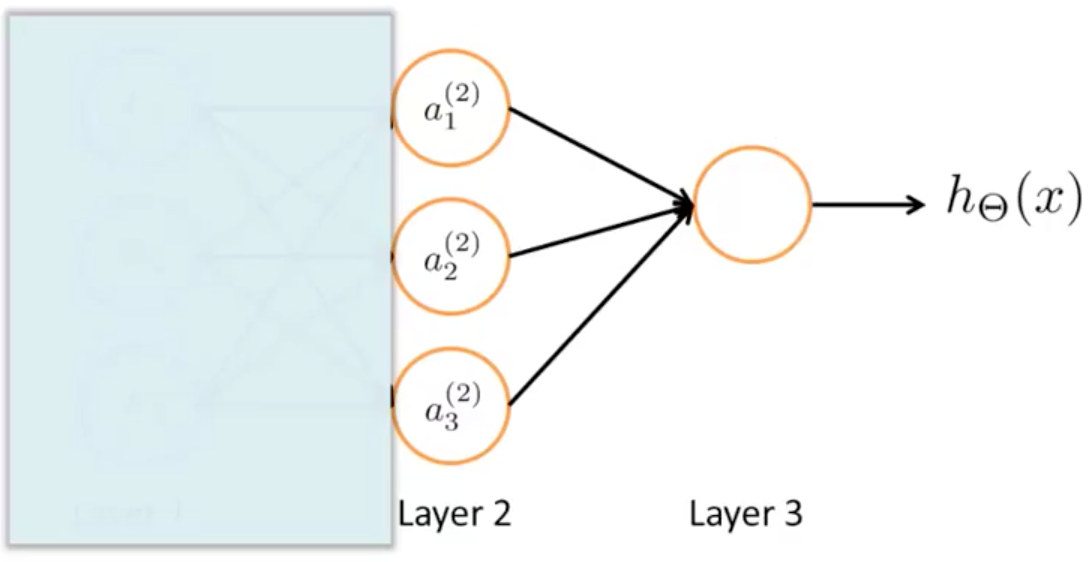
\includegraphics[scale=0.15]{images/logisticnet}
		\caption*{(a)}
	\end{minipage}%
	\hspace{4mm}%
	\begin{minipage}[c]{.43\textwidth}
		\centering
		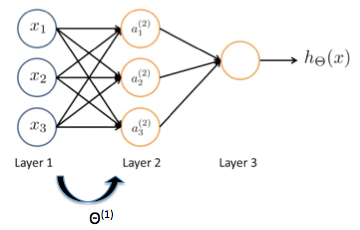
\includegraphics[scale=0.45]{images/logisticnet2}
		\caption*{(b)}
	\end{minipage}
	\caption{An example of neural network}
	\label{logisticnet}
\end{figure}

%\begin{figure}[H]
%\begin{center}
%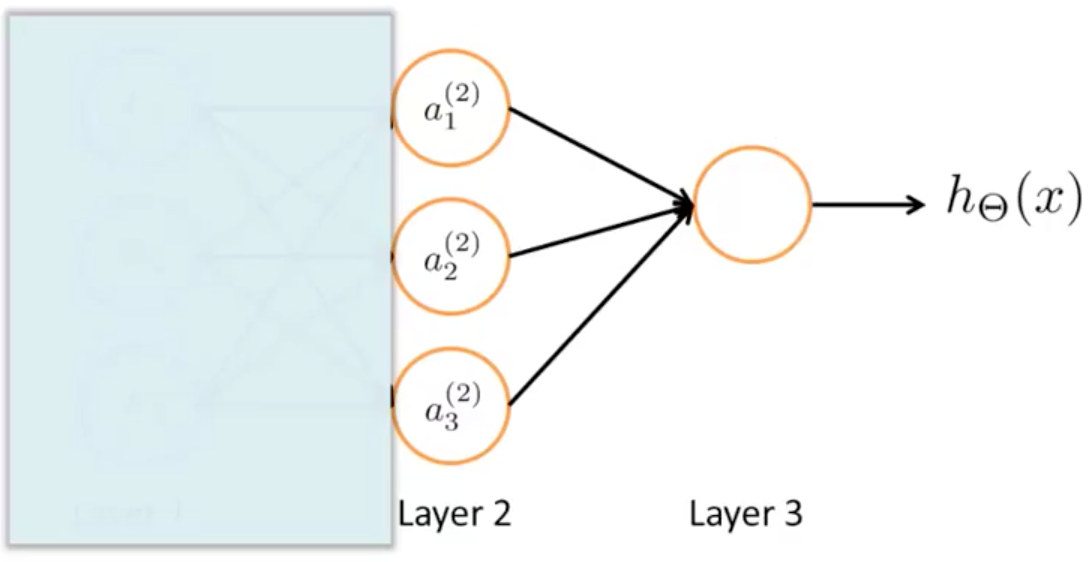
\includegraphics[scale=0.25]{images/logisticnet}
%\end{center}
%\caption{An example of neural network} 
%\label{logisticnet}
%\end{figure}

If we look at figure \ref{logisticnet}-a it looks like a logistic regression unit able to predict $h_{\Theta}(x)$, where:

\begin{eqfloat}[H]
\begin{equation}
	h_{\Theta}(x) = g( \Theta_{0}a_0^{(2)} + \Theta_{1}a_1^{(2)} +  \Theta_{2}a_2^{(2)} + \Theta_{3}a_3^{(2)} )
\end{equation}
      \addtocounter{equation}{-1}
        \caption{  Hypothesis function}
        \label{eq:logistic}
    \end{eqfloat}



If in equation \ref{eq:logistic} we do not consider the superscript $(2)$, it looks like the standard logistic regression equation except that now we are using $\Theta$ instead of $\theta$; in this case the input features of the logistic regression are the values computed by the hidden layer. In fact, the represented neural network is doing a logistic regression computation using $a_1^{(2)}$, $a_2^{(2)}$, $a_3^{(2)}$  rather than use the original features  $x_1$, $x_2$, $x_3$. The interesting thing is that the features $a_1^{(2)}$, $a_2^{(2)}$, $a_3^{(2)}$ are themselves learned as functions of the input $x_1$, $x_2$, $x_3$. Concretely the function mapping from layer 1 to layer 2 is determined by other set of parameters $\Theta^{(1)}$. So, that shows how a neural network instead of being constrained to feed the features $x_1$, $x_2$, $x_3$ to logistic regression, it gets to learn its own features $a_1^{(2)}$, $a_2^{(2)}$, $a_3^{(2)}$ to feed into logistic regression and depending on what parameters it chooses for $\Theta_1$ it can learn some pretty interesting and complex features and therefore we can obtain a better hypothesis than if we were constrained to use the raw features $x_1$, $x_2$, $x_3$. This algorithm has the flexibility to try to learn whatever features at once using $a_1^{(2)}$, $a_2^{(2)}$, $a_3^{(2)}$ in order to feed the output unit $h_\Theta(x)$. This example is described at high level, so to better understand the intuition beyond the neural networks, in the following we'll see some examples.


\begin{mydef}
{\bf Architecture of a Neural Network:} how the different neurons of a network are connected each others.
\end{mydef}



\subsection{Examples and Intuitions}

In the following some examples how neural networks can compute complex non-linear hypotheses are reported. Consider the following example with input features $x_1$ and $x_2$ that are binary values $(0,1)$.

\begin{figure}[H]
\begin{center}
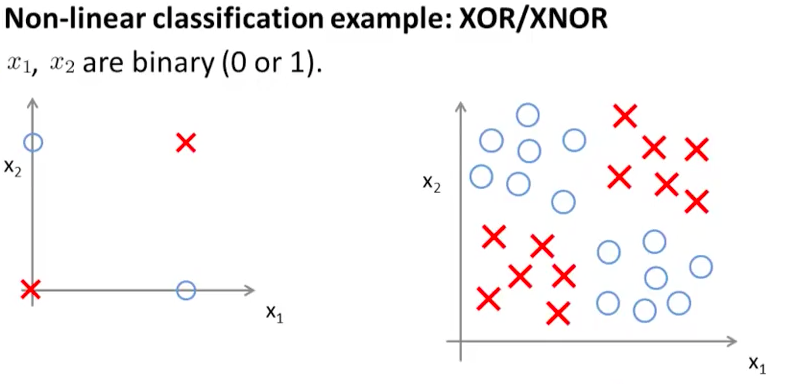
\includegraphics[scale=0.25]{images/xor}
\end{center}
\caption{Non-linear Classification example: XOR/XNOR } 
\label{xor}
\end{figure}

In figure \ref{xor}, on the left we have a simplified version of a more complex (on the right) learning problem. We would like to learn a non-linear function (decision boundary) to separate positive and negative examples. Looking at the simplified version we can consider positive examples ($y=1$, the X symbol) if both $x_1$ and $x_2$ are equal to zero or if $x_1 = x_2 = 1$. We want to figure out if we can get a neural network to fit the training set of the example. Before to build the neural network that fit the above example (that is a XNOR function), let's start building a neural network that fits the AND logic function at first and then some other logic functions.

\newpage
\begin{mdframed}[style=MyFrame]
\subsubsection{Example1:  AND Neural Network}


\begin{wrapfigure}{l}{4.5cm}
\begin{center}
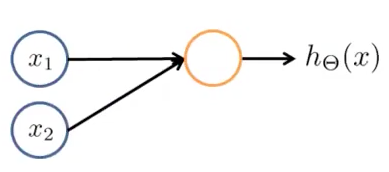
\includegraphics[scale=0.25]{images/and1}
\end{center}
\caption{Non-linear Classification example: AND} 
\label{and1}
\end{wrapfigure}

In figure \ref{and1} we have a unit network to compute the {\bf logical AND}:
\begin{itemize}
\item $x_1, x_2 \in \{0,1\}$
\item $y = x_1 \land x_2$
\end{itemize}

Let's add the bias unit and assign some values to the weights (parameters) of the network (figure \ref{and2}):

\begin{figure}[H]
\begin{center}
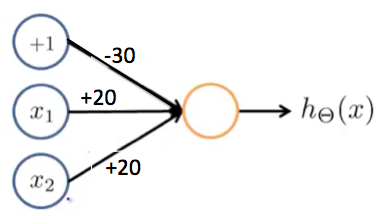
\includegraphics[scale=0.25]{images/and2}
\end{center}
\caption{Non-linear Classification example with bias unit and weights: AND} 
\label{and2}
\end{figure}


Given the neural network represented in figure \ref{and2}, the hypothesis $h_\Theta(x)$ will be:

\begin{eqfloat}[H]
\begin{equation}
	h_{\Theta}(x) = g(-30 + 20x_1 + 20x_2 ) 
\end{equation}
      \addtocounter{equation}{-1}
        \caption{  AND Hypothesis function}
        \label{eq:andhyp}
\end{eqfloat}

where:

\begin{itemize}
\item $\Theta_{10}^{(1)} = -30$
\item $\Theta_{11}^{(1)} = +20$
\item $\Theta_{12}^{(1)} = +20$
\end{itemize}

Taking into account the sigmoid function $g(z)$ represented in figure \ref{sigmoidplot}, look at the four possible input values for $x_1$ and $x_2$ 
 
 
 \begin{figure}[H]
\begin{center}
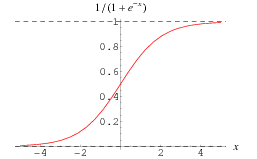
\includegraphics[scale=0.60]{images/sigmoidplot}
\end{center}
\caption{Sigmoid function $g(z)$} 
\label{sigmoidplot}
\end{figure}


\begin{table}[H]
\caption{Table related to neural network in figure \ref{and2} (Logic AND) }
\centering
\begin{tabular}{c c c }
\hline\hline
$x_1$	&	$x_2$ & $h_{\Theta}(x) = g(-30 + 20x_1 + 20x_2 ) $ \\ [0.5ex] % inserts table %heading
\hline
$0$ &	$0$	& $g(-30) \approx 0$ \\
$0$ &	$1$	& $g(-30 + 20) \approx 0$ \\
$1$ &	$0$	& $g(-30 + 20) \approx 0$ \\
$1$ &	$1$	& $g(-30 + 20 +20) \approx 1$ \\
\hline
\end{tabular}
\label{table:nov-ser}
\end{table}
\end{mdframed}


%%%%%%%%%%%%%%%%%%%%%%%%%%%%%
\newpage
\begin{mdframed}[style=MyFrame]
\subsubsection{ Example2:  NOT Neural Network}

\begin{eqfloat}[H]
\begin{equation}
\begin{aligned}
x_1 \in \{0,1\} \\
h_{\Theta}(x) = g(10 - 20x_1) 
\end{aligned}
\end{equation}
      \addtocounter{equation}{-1}
        \caption{  NOT Hypothesis function}
        \label{eq:nothyp}
    \end{eqfloat}


%%%%%%%%%%%%%%%%%%%%%%%%%%%%%%%%OK multiple figure
\begin{figure}[H]
	\centering
	\begin{minipage}[c]{.43\textwidth}
		\centering
		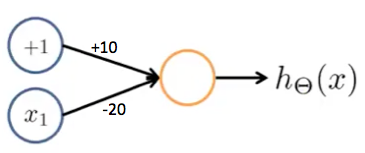
\includegraphics[scale=0.45]{images/not}
		\caption*{(a)}
	\end{minipage}%
	\hspace{4mm}%
	\begin{minipage}[c]{.43\textwidth}
		\centering
		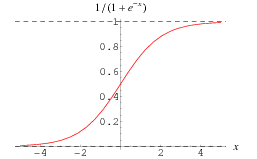
\includegraphics[scale=0.50]{images/sigmoidplot}
		\caption*{(b)}
	\end{minipage}
	\caption{Non-linear Classification example: NOT(a) and Sigmoid function $g(z)$ (b)}\label{fig:not}
\end{figure}


\begin{table}[H]
\caption{Table related to neural network in figure \ref{fig:not}-a (Logic NOT) }
\centering
\begin{tabular}{c c }
\hline\hline
$x_1$	&  $h_{\Theta}(x) = g(10 - 20x_1 )$  \\ [0.5ex] % inserts table %heading
\hline
$0$ 	& $g(10) \approx 1$ \\
$1$ 	& $g(+10 - 20) \approx 0$ \\
\hline
\end{tabular}
\label{table:nov-ser}
\end{table}

\end{mdframed}


%%%%%%%%%%%%%%%%%%%%%%%%%%%%%
\begin{mdframed}[style=MyFrame]
\subsubsection{ Example3:  (NOT ) AND (NOT) Neural Network}



\begin{figure}[H]
	\centering
	\begin{minipage}[c]{.46\textwidth}
		\centering
		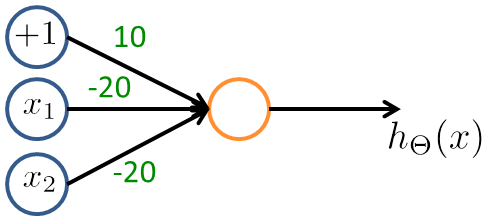
\includegraphics[scale=0.35]{images/notx1andnotx2}		
	\end{minipage}%
	\hspace{4mm}%
	\begin{minipage}[c]{.46\textwidth}
		\centering
		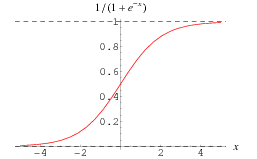
\includegraphics[scale=0.55]{images/sigmoidplot}
	\end{minipage}
	\caption{(NOT) AND (NOT) Neural Network example}\label{fig:notx1andnotx2}
\end{figure}

\begin{table}[H]
\caption{Table related to neural network in figure \ref{fig:notx1andnotx2} ((NOT $x_1$) AND (NOT $x_2$)) }
\centering
\begin{tabular}{c c c }
\hline\hline
$x_1$	&	$x_2$ & $h_{\Theta}(x) = g(10 - 20x_1 - 20x_2 )$  \\ [0.5ex] % inserts table %heading
\hline
$0$ &	$0$	& $g(10) \approx 1$ \\
$0$ &	$1$	& $g(+10 - 20) \approx 0$ \\
$1$ &	$0$	& $g(+10 - 20) \approx 0$ \\
$1$ &	$1$	& $g(+10 - 20 - 20) \approx 0$ \\
\hline
\end{tabular}
\label{table:nov-ser}
\end{table}
\end{mdframed}


%%%%%%%%%%%%%%%%%%%%%%%%%%%%%
\newpage
\begin{mdframed}[style=MyFrame]
\subsubsection{Example 4:  OR Neural Network}

\begin{figure}[H]
	\centering
	\begin{minipage}[c]{.46\textwidth}
		\centering
		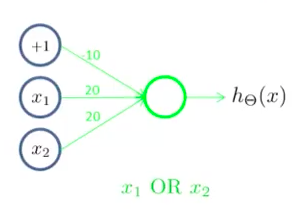
\includegraphics[scale=0.35]{images/or}		
	\end{minipage}%
	\hspace{4mm}%
	\begin{minipage}[c]{.46\textwidth}
		\centering
		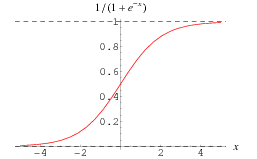
\includegraphics[scale=0.55]{images/sigmoidplot}
	\end{minipage}
	\caption{OR Neural Network example}\label{fig:notx1andnotx2}
	 \label{fig:or}%
\end{figure}




\begin{table}[H]
\caption{Table related to neural network in figure \ref{fig:or} $x_1$ OR  $x_2$ }
\centering
\begin{tabular}{c c c }
\hline\hline
$x_1$	&	$x_2$ & $h_{\Theta}(x) = g(-10 + 20x_1 + 20x_2 )$  \\ [0.5ex] % inserts table %heading
\hline
$0$ &	$0$	& $g(-10) \approx 0$ \\
$0$ &	$1$	& $g(-10 + 20) \approx 1$ \\
$1$ &	$0$	& $g(-10 + 20) \approx 1$ \\
$1$ &	$1$	& $g(-10 + 20 + 20) \approx 1$ \\
\hline
\end{tabular}
\label{table:nov-ser}
\end{table}
\end{mdframed}



\subsubsection{ XNOR  Neural Network}
Now we want to put together the neural networks we have seen previously in order to compute $x_1$ XNOR $x_2$. So, starting from the training example in figure ~\ref{fig:xor1-xnor}, we need a decision boundary in order to separate positive and negative examples. In figure \ref{fig:xnor} the related neural network is represented.


\begin{figure}[H]
\begin{center}
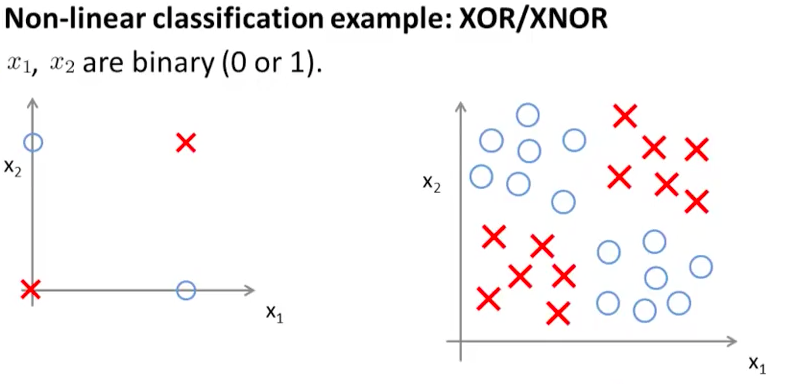
\includegraphics[scale=0.25]{images/xor}
\end{center}
\caption{Non-linear Classification example: XOR/XNOR } 
\label{fig:xor1-xnor}
\end{figure}


\begin{figure}[H]
\begin{center}
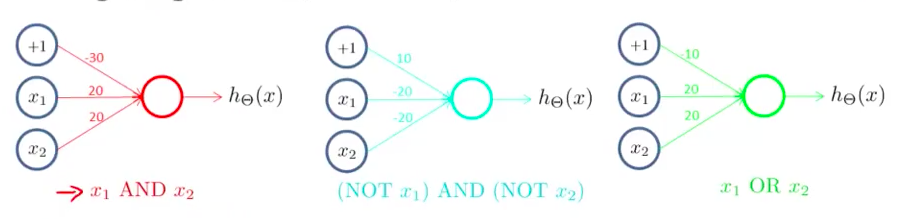
\includegraphics[scale=0.35]{images/all-logic}
\end{center}
\caption{Non-linear Classification examples } 
\label{xor1}
\end{figure}



\begin{figure}[H]
	\centering
	\begin{minipage}[c]{.46\textwidth}
		\centering
		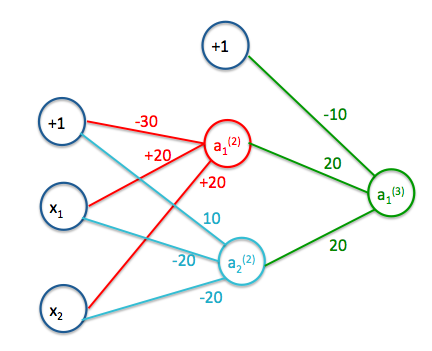
\includegraphics[scale=0.35]{images/xnor}		
	\end{minipage}%
	\hspace{4mm}%
	\begin{minipage}[c]{.46\textwidth}
		\centering
		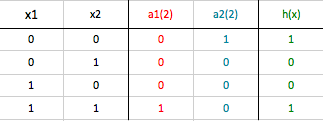
\includegraphics[scale=0.55]{images/xnor-table}
	\end{minipage}
	\caption{Non-linear Classification example: XNOR}\label{fig:xnor}
\end{figure}


So, we can notice that $h_\Theta(x) = 1$ if $x_1 = x_2 = 0$ or if $x_1 = x_2 = 1$ (see figure \ref{fig:xnor}); in this way we found a non-linear decision boundary that computes the nor function. \\
The general intuition is that in the input layer we have the raw inputs, then a hidden layer  is added in order to compute some slightly more complex functions (and, or, etc.) of the inputs and, finally, the output layer computes an even more complex non-linear function.

In general we can state that the deeper the layer is, more complicated the computed non-linear function is.


\subsection{Multiclass classification}
This section explains how to use neural networks to do multiples classification by means of an extension of the one-vs-all method. 

Let's consider a computer vision example where we want to recognize four categories of objects (given an image): pedestrian, car, motorcycle, truck.
We would build a a neural network with four output units, so that the output is a vector of four numbers ($h_\Theta(x) \in \mathbb{R}^4$); so, in this example the network has four output units where:

\begin{itemize}
\item output unit 1: predict if the image is a pedestrian or not;
\item output unit 2: predict if the image is a car or not;
\item output unit 3: predict if the image is a motorcycle or not;
\item output unit 4: predict if the image is a truck or not;
\end{itemize}


The four output units could be seen as four logistic regression classifier.

\begin{figure}[H]
\begin{center}
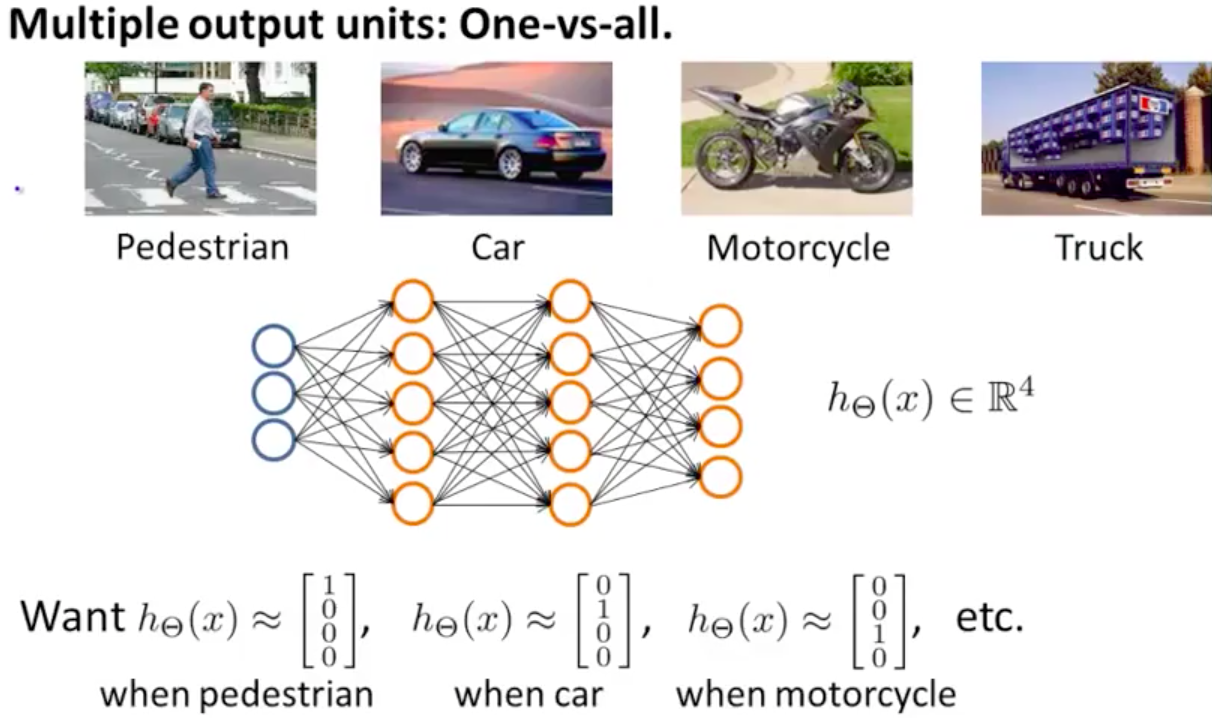
\includegraphics[scale=0.25]{images/one-vs-all-ex}
\end{center}
\caption{Multi-class classification example: one-vs-all } 
\label{xor1}
\end{figure}

\newpage
\begin{mdframed}[style=MyFrame]
\subsubsection{Exercise}
Suppose you have a multi-class classification problem with 10 classes. Your neural network has 3 layers, and the hidden layer (layer 2) has 5 units. Using the one-vs-all method how many elements does $\Theta^{(2)}$ has?\\


\subsubsection{Solution}
In general :\\
$\Theta^{(j)} \in (S_{j+1}) \times (S_j +1)$;\\
where $S_j$ is the number of units in layer $j$.\\
\\
We have:
\begin{itemize}
	\item layer 2 $\Rightarrow$ 5 units
	\item output layer (layer 3) $\Rightarrow$ 10 units
\end{itemize}
So, \\
$\Theta^{(2)} \in (S_{3}) \times (S_2 +1) = 10 \times 6$ 
\end{mdframed}

\subsection{Neural Networks: learning. Cost function}
This section studies how to learn the parameters of a neural network given a training set. Suppose to have the following neural network:

\begin{figure}[H]
\begin{center}
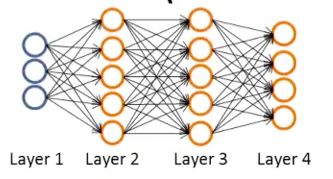
\includegraphics[scale=0.35]{images/learn-nn}
\end{center}
\caption{Multi-class classification neural network example } 
\label{fig:learn-nn}
\end{figure}
 
and that:
\begin{itemize}
	\item $\{ (x^{(1)},y^{(1)}), (x^{(2)},y^{(2)}), \hdots, (x^{(m)},y^{(m)}) \}$ is the training set;
	\item $L$ is the total number of layer in the considered network ($L = 4$ in the above example);
	\item $S_l$ is the number of units in layer $l$.\\
\end{itemize}

In the example two types of classification problems are considered:
\begin{itemize}
	\item {\it Binary classification}: $y \in \{0,1\} $
	\item {\it Multi-class classification}(K-classes):
	\begin{itemize}
		\item $y \in \mathbb{R}^k$;
		\item $k$ output units;
	\end{itemize}
\end{itemize}


The cost function for the above neural network can be defined as a generalization of the logistic regression cost function:



\begin{eqfloat}[H]
\begin{equation}
	J(\Theta)  = -\frac{1}{m}[ \sum_{i=1}^{m} y^{(i)} \log h_\Theta(x^{(i)}) + (1 - y^{(i)}) \log (1 - h_\Theta(x^{(i)}) )] + \frac{\lambda}{2m}\sum_{j=1}^{n} \Theta_j^2
\end{equation}
      \addtocounter{equation}{-1}
        \caption{ Logistic Regression Cost function.}
        \label{eq:logregcostfunc}
    \end{eqfloat}


{\bf Note that the regularization is not applied to $\Theta_0$}.

In the case of neural networks the cost function  is a generalization of the logistic regression one (equation ~\ref{eq:logregcostfunc}), where instead of having just one logistic regression output unit, there may be $k$ output units, so the cost function is:


\begin{eqfloat}[H]
\begin{equation}
\begin{aligned}
J(\Theta)  = -\frac{1}{m}[ \sum_{i=1}^{m} \sum_{k=1}^{K} y^{(i)}_k \log (h_\Theta(x^{(i)}))_k + (1 - y^{(i)}_k) \log (1 - (h_\Theta(x^{(i)}) )_k)] \\ 
+ \frac{\lambda}{2m} 
\sum_{l=1}^{L} 
\sum_{i=1}^{S_l} 
\sum_{j=1}^{S_{l+1}} (\Theta_{ij}^{(l)})^2
\end{aligned}
\end{equation}
      \addtocounter{equation}{-1}
        \caption{ Neural Networks Cost function.}
        \label{eq:nncostfunc}
    \end{eqfloat}



Where :
\begin{itemize}
		\item $h_\Theta(x) \in \mathbb{R}^K$;
		\item $(h_\Theta(x))_i = i^{th}$ output.
	\end{itemize}
	
Observing the regularization term 
$\frac{\lambda}{2m} 
\sum_{l=1}^{L} 
\sum_{i=1}^{S_l} 
\sum_{j=1}^{S_{l+1}} (\Theta_ij^{(l)})^2$	
can be noticed that the sum is built by summing over $\Theta_{ij}^{(l)}$ for all $i,j$ and $l$ except that for the terms that correspond to the bias values; Concretely, the sum does not consider the case of $i=0$. The reason why that terms are not considered is that they would be multiplied with the bias units.


\subsection{Backpropagation algorithm}
Now, the {\bf backpropagation algorithm} that aims to minimize the cost function is presented. In order to minimize the cost function through the {\bf gradient descent} or some other {\bf optimization algorithms}, we need to implement the code that take the parameter $\Theta$ as input and compute $J(\Theta)$ and the partial derivatives terms (remember that the gradient descent is an algorithm that uses the partial derivatives in order to find the local minimum of a function):


\begin{eqfloat}[H]
\begin{equation}
\frac{\partial}{\partial \Theta_{ij}^{(l)}} J(\Theta)
\end{equation}
      \addtocounter{equation}{-1}
        \caption{ Partial Derivatives terms.}
        \label{eq:partderiv}
    \end{eqfloat}


Now, let's focus on the computation of the partial derivatives. Consider the case where only one training example $(x,y)$ is available. First of all we have to apply the forward propagation in order to compute what the hypothesis outputs given an input feature $x$:

\begin{eqfloat}[H]
\begin{equation}
	\begin{aligned}
	a^{(1)}  = x \\
	z^{(2)}  = \Theta^{(1)}a^{(1)} \\
	a^{(2)}  = g(z^{(2)}) \text{ add }  a_0^{(2)} \\
	z^{(3)}  = \Theta^{(2)}a^{(2)} \\
	a^{(3)}  = g(z^{(3)}) \text{ add }  a_0^{(3)} \\
	z^{(4)}  = \Theta^{(3)}a^{(3)} \\
	a^{(4)}  = g(z^{(4)}) = h_\Theta(x)
	\end{aligned}	
\end{equation}
      \addtocounter{equation}{-1}
        \caption{ Forward propagation application - vectorized implementation}
        \label{eq:forwprop}
    \end{eqfloat}

The vectorized implementation of the forward propagation algorithm allows us to compute all  {\bf activation values} for all neurons of the neural network. In order to compute the derivatives we use the {\bf Backpropagation algorithm}. 


\subsubsection{Gradient computation: Backpropagation algorithm}
Before to see the backpropagation algorithm, let's define  $\delta$:\\
\begin{mydef}
$\delta_j^{(l)}$: Error of node $j$ in layer $l$ (it can be defined as the difference between the hypothesis output $h_\Theta(x)$ and the real output value $y$)
\end{mydef}

The backpropagation algorithm is based on the intuition that for each node $j$ of the neural network, the value $\delta_j^{(l)}$, that represents the error of the node $j$ in layer $l$ is computed.

Remember that :\\
$a_j^{(j)}$ is the activation of unit $j$ in layer $l$.


\begin{figure}[H]
\begin{center}
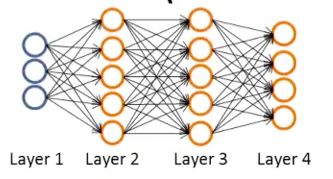
\includegraphics[scale=0.35]{images/learn-nn}
\end{center}
\caption{Multi-class classification neural network example } 
\label{fig:learn-nn1}
\end{figure}

Consider the neural network in figure \ref{fig:learn-nn1}; we have four layers ($L=4$) and for each output unit we have to compute: $\delta_j^{4} = a_j^{(4)} - y_j$ where $a_j^{(4)} = (h_\Theta(x))_j$. If we think of $\delta$, $a$ and $y$ as vectors, we can use the vectorized implementation:

\begin{eqfloat}[H]
\begin{equation}
\delta^{(4)} = a^{(4)} - y 	\qquad \qquad 	\delta^{4}, a^{(4)}, y \in \mathbb{R}^L 
\end{equation}
      \addtocounter{equation}{-1}
        \caption{ Error computation with vectorized implementation}
        \label{eq:errvect}
    \end{eqfloat}

where  $L$ is the number of output units.


The next step is the computation of the $\delta$ terms for the earlier layers in the network:

\begin{eqfloat}[H]
\begin{equation}
	\begin{aligned}
	\delta^{(3)} = (\Theta^{(3)})^T  \delta^{(4)} .* g^{\prime}(z^{(3)})\\
	\delta^{(2)} = (\Theta^{(2)})^T  \delta^{(3)} .* g^{\prime}(z^{(2)})
	\end{aligned}	
\end{equation}
      \addtocounter{equation}{-1}
        \caption{ Error computation with vectorized implementation for the other layers of the network}
        \label{eq:errcomp}
    \end{eqfloat}


where $g^{\prime}(z^{(l)})$ is the derivative of the activation function $g$ evaluated at the input value given by $z^{(l)}$, and it is computes as follows:

\begin{eqfloat}[H]
\begin{equation}
	g^{\prime}(z^{(l)}) = a^{(l)} .* (1 - a^{(l)})
\end{equation}
      \addtocounter{equation}{-1}
        \caption{ Error computation with vectorized implementation for the other layers of the network}
        \label{eq:errcomp}
    \end{eqfloat}
where:
\begin{itemize}
	\item $a^{(l)}$ is a vector of activations;
	\item $1$ is a vector of $1_s$
\end{itemize}

\begin{mydef} 
The symbol ``.* '' is the notation for the element wise multiplication, also called {\it Hadamard product}. It is a binary operation that takes two matrices of the same dimensions, and produces another matrix where each element $ij$ is the product of elements $ij$ of the original two matrices.
\end{mydef} 

Note that there is not $\delta^{(1)}$ term because the first layer corresponds to the input layer where the values are the features observed in the training set, so there isn't any prediction error associated to them.

It is possible to proof that the partial derivative terms is given by

\begin{eqfloat}[H]
\begin{equation}
\frac{\partial}{\partial \Theta_{ij}^{(l)}} J(\Theta) = a_j^{(j)} \delta_i^{(l+1)}
\end{equation}
      \addtocounter{equation}{-1}
        \caption{ Partial Derivatives terms computation (case of one training examples)}
        \label{eq:partderivcomp}
    \end{eqfloat}

Till now we considered the case of a single training example; in the following we will put all together to see how to implement the {\bf backpropagation algorithm} to compute the derivatives with respect to the parameters and for those cases characterized by a large training set.


Suppose to have a training set of m examples:\\

$\{ (x^{(1)},y^{(1)} ), (x^{(2)},y^{(2)} ), \hdots, (x^{(m)},y^{(m)} ) \}$

we can implement the backpropagation algorithm as follows:


\begin{algorithm}
\footnotesize
\caption{Backpropagation algorithm}\label{backpropalg}
\label{algorithm}
\begin{algorithmic}[1]
\State Set $\Delta_{ij}^{(l)} = 0$ for all $i,j,l$;
\For {$i=1\dots m}$
	\State Set  $a^{(1)} = x^{(i)}$  %\Comment  User 1
	\State Perform forward propagation to compute $a^{(l)}$ for $l=2,3, \hdots, L$
	\State Using $y^{(i)}$, compute $\delta^{(L)} = a^{(L)} - y^{(i)}$	
	\State Compute  $\delta^{(L-1)},\delta^{(L-2)}, \hdots, \delta^{(2)}$
	\State $\Delta_{ij}^{(l)} := \Delta_{ij}^{(l)} + a_j^{(l)}\delta_i^{(l+1)}$
\EndFor
\State $D_{ij}^{(l)} := \frac{1}{m} \Delta_{ij}^{(l)} + \frac{\lambda \Theta_{ij}^{(l)}}{m}$  if $j\neq0$
\State $D_{ij}^{(l)} := \frac{1}{m} \Delta_{ij}^{(l)}$  if $j = 0$
\end{algorithmic}
\end{algorithm}

Note that $j = 0$ corresponds to the bias term, that is why we are omitting the regularization term. The formal proof is quite complicate (and we omit that), but we can state that:


\begin{eqfloat}[H]
\begin{equation}
\frac{\partial}{\partial \Theta_{ij}^{(l)}} J(\Theta) = D_{ij}^{(l)}
\end{equation}
      \addtocounter{equation}{-1}
        \caption{ Partial Derivatives terms computation (case of multiple training examples) }
        \label{eq:partderivcomp1}
    \end{eqfloat}


We can use equation ~\ref{eq:partderivcomp1} with either gradient descent or in one of the advanced optimization algorithms.
\\
Now we are going to analyze the mechanical steps of the backpropagation algorithm, but to better understand this algorithm, let's take a look at what forward propagation does (see figure \ref{fig:forwpropcomp}), particularly we take into account the computation of the $z_1^{(3)}$ activation.



\begin{figure}[H]
\begin{center}
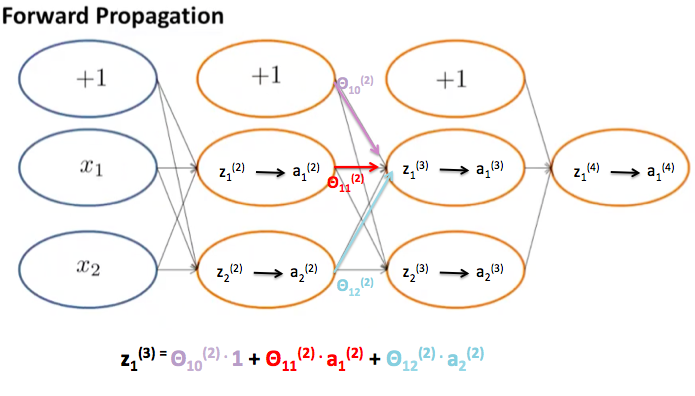
\includegraphics[scale=0.35]{images/forwpropcomp}
\end{center}
\caption{Forward propagation computation } 
\label{fig:forwpropcomp}
\end{figure}


What backpropagation does is very similar to what we have seen for forward propagation, except that instead of perform the computation flowing from left to the right, it flows from the right to the left. In order to understand the backpropagation algorithm, let's observe the cost function for the case where we have just one output unit (equation ~\ref{eq:nncostfunc1}):


\begin{eqfloat}[H]
\begin{equation}
\begin{aligned}
J(\Theta)  = -\frac{1}{m}[ \sum_{i=1}^{m} \sum_{k=1}^{K} y^{(i)}_k \log (h_\Theta(x^{(i)}))_k + (1 - y^{(i)}_k) \log (1 - (h_\Theta(x^{(i)}) )_k)] \\ 
+ \frac{\lambda}{2m} 
\sum_{l=1}^{L} 
\sum_{i=1}^{S_l} 
\sum_{j=1}^{S_{l+1}} (\Theta_{ij}^{(l)})^2
\end{aligned}
\end{equation}
      \addtocounter{equation}{-1}
        \caption{ Neural Networks Cost function.}
        \label{eq:nncostfunc1}
    \end{eqfloat}
    
    
If we focus on the case of a single training example $(x^{(i)}, y^{(i)})$, one output unit and ignore the regularization     term $(\lambda = 0)$ , we obtain the following cost function:

\begin{eqfloat}[H]
\begin{equation}
	cost(i)  =  y^{(i)} \log h_\Theta(x^{(i)}) + (1 - y^{(i)}) \log h_\Theta(x^{(i)})  \\ 
\end{equation}
      \addtocounter{equation}{-1}
        \caption{ Neural Networks Cost function, one single example, one out unit and no regularization}
        \label{eq:nncostfunc2}
    \end{eqfloat}

$cost(i)$ is the cost associated with the $i^{th}$ example and we can think to that as: $cost(i)  \simeq  (h_\Theta(x^{(i)}) - y^{(i)})^2$, so it plays a role similar to the square error.

As in the case of logistic regression, in neural networks we use a slightly more complicated function using the logarithm. So, the cost function $cost(i)$ measures how well the neural network is doing on correctly predicting the example $i$.

An intuition is that the {\bf backpropagation algorithm} computes the error $\delta_j^{(l)}$ that is the error  of the activation value of the unit $a_j^{(l)}$ (unit $j$ of the layer $l$). More formally:

\begin{eqfloat}[H]
\begin{equation}
\delta_j^{(l)}  = \frac{\partial}{\partial z_j^{(l)}} cost(i)  \qquad \text{for } j >= 0 
\end{equation}
      \addtocounter{equation}{-1}
        \caption{ Error of the activation value of unit j in layer l}
        \label{eq:deltaerror}
    \end{eqfloat}
    
    where:
    \begin{eqfloat}[H]
\begin{equation}
	cost(i)  =  y^{(i)} \log h_\Theta(x^{(i)}) + (1 - y^{(i)}) \log h_\Theta(x^{(i)})  \\ 
\end{equation}
      \addtocounter{equation}{-1}
        \caption{  Cost function of the activation unit}
        \label{eq:nncostfunc3}
    \end{eqfloat}
    
In the following, more details about what the backpropagation algorithm does are given:

\begin{itemize}    
\item For the output layer the error is given by $\delta_1^{(4)} = y^{(i)} - a_1^{(4)}$, which is the error measured as the difference between the actual value $y^{(i)}$ and the predicted value $a_1^{(4)}$.
\item Next, the computed value $\delta_1^{(4)}$ is propagated backward in previous layer and  the delta terms for the previous layer ($\delta_1^{(3)}$,$\delta_2^{(3)}$ ) are computed.
\item The algorithm follows by propagating backward in the previous layers and computing $\delta_1^{(2)}$,$\delta_2^{(2)}$.
\end{itemize}    
    
The backpropagation computation is like running the forward propagation algorithm, but doing it backwards.         


\subsection{Neural networks: implementation notes}
In this section we will see some Matlab implementation details about {\bf unrolling} the parameters from matrices into vectors, in order to use the advances optimization routines.

In neural networks, parameters are no longer vectors (as in logistic regression), but are matrices:

{\bf Neural Network L=4}:
\begin{itemize}
\item $\Theta^{(1)}, \Theta^{(2)}, \Theta^{(3)}$ - Matrices (Theta1, Theta2, Theta3);
\item $D^{(1)}, D^{(2)}, D^{(3)}$ - Matrices (D1, D2, D3);
\end{itemize}

We want to {\bf unroll} these matrices into vectors so that they end up being in a format suitable for passing as parameters in the implementation of the cost function:
%\newpage
\begin{mdframed}[style=MyFrame]
\begin{lstlisting}
function [jVal, gradient] = costFunction(theta)
...
optTheta = fminunc(@costFunction, initialTheta, options)  
\end{lstlisting}
\end{mdframed}
Note that $theta \in \mathbb{R}^{n+1}$ and $initialTheta \in \mathbb{R}^{n+1}$ are vectors.


\begin{wrapfigure}{l}{4.5cm}
\begin{center}
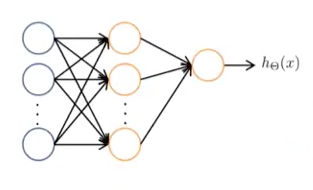
\includegraphics[scale=0.35]{images/nnunrollex}
\end{center}
\caption{Forward propagation computation } 
\label{fig:nnunrollex}
\end{wrapfigure}

Concretely, if we have a neural network with a input layer that has 10 units, one hidden layer with 10 units and one output layer with 1 unit (like that represented in figure \ref{fig:nnunrollex}), we have the following parameters:

\begin{itemize}
\item $S_1 = 10, S_2 = 10, S_3 = 1$\\
\item $\Theta^{(1)} \in  \mathbb{R}^{10 \times 11}, \Theta^{(2)} \in  \mathbb{R}^{10 \times 11}, \Theta^{(3)} \in  \mathbb{R}^{1 \times 11}$\\
\item $D^{(1)} \in  \mathbb{R}^{10 \times 11}, D^{(2)} \in  \mathbb{R}^{10 \times 11}, D^{(3)} \in  \mathbb{R}^{1 \times 11}$\\
\end{itemize}

In Matlab, in order to obtain the vectors starting from the matrices we have to run the following code:

\begin{mdframed}[style=MyFrame]
\begin{lstlisting}
thetaVec = [Theta1(:) ; Theta2(:) ; Theta3(:)];
DVec = [D1(:) ; D2(:) ; D3(:)];
\end{lstlisting}
\end{mdframed}

The above code will unroll all the element of the matrices {\bf Theta1, Theta2, Theta3} in a big long vector called {\bf thetaVec}. In the same way we created the vector {\bf DVec}.

If we want to go back from the vector representation, to the original matrix representation we have to run the following code:

\begin{mdframed}[style=MyFrame]
\begin{lstlisting}
Theta1 = reshape(thetaVec(1:110),10,11)
Theta2 = reshape(thetaVec(111:220),10,11)
Theta1 = reshape(thetaVec(221:231),1,11)
\end{lstlisting}
\end{mdframed}


In the following all steps needed to implement a learning algorithm are summarized:

\begin{algorithm}[H]
\footnotesize
\caption{Learning algorithm}
\label{learnalg}
\begin{algorithmic}[1]
\State Suppose to have initial parameters $\Theta^{(1)}, \Theta^{(2)}, \Theta^{(3)}$;  %\Comment  User 1
\State Unroll $\Theta^{(1)}, \Theta^{(2)}, \Theta^{(3)}$ to get {\bf initialTheta} to pass to: 
\begin{lstlisting}
fminunc(@costFunction, initialTheta, options)  
\end{lstlisting}
\State the other thing to do is the implementation of the {\bf cost function}:
%\State 
\begin{lstlisting}
function [jVal, gradient] = costFunction(thetaVec)
\end{lstlisting}
\State from {\bf thetaVec}, get $\Theta^{(1)}, \Theta^{(2)}, \Theta^{(3)}$ \Comment Using the {\bf reshape function}
\State Use {\bf forward prop} / {\bf back prop} to compute $D^{(1)}, D^{(2)}, D^{(3)}$ and $J(\Theta)$.
\State unroll $D^{(1)}, D^{(2)}, D^{(3)}$ to get {\bf gradientVec}.
\end{algorithmic}
\end{algorithm}

Summarizing:

\begin{itemize}
\item parameters in {\bf matrix representation}: more convenient to do backpropagation and forward propagation;
\item parameters in {\bf vector representation}: more convenient for the advanced optimization algorithms.
\end{itemize}


\subsection{Gradient Checking}

Sometimes we could implement a back propagation algorithm that led to a decreasing of the cost function $J(\Theta)$ but that contains some errors. Given the decreasing of the cost function, it could be difficult to see the error, so we end up to implement a neural network that contain a high level of error.

In order to avoid the just described problem we can use the {\bf gradient checking} algorithm. In fact, once we implement the numerical gradient checking we are able to verify if our back propagation implementation is really computing the derivatives of the cost function $J(\Theta)$.

\begin{wrapfigure}{l}{5cm}
\begin{center}
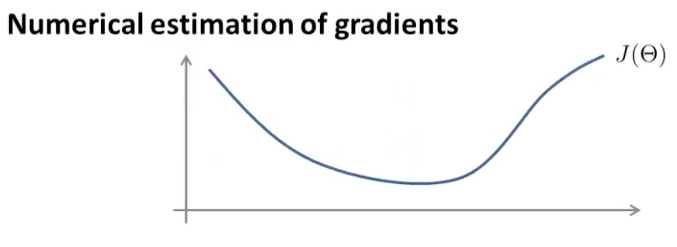
\includegraphics[scale=0.2]{images/gradcheck}
\end{center}
\caption{Cost function example } 
\label{fig:gradcheck}
\end{wrapfigure}

Suppose to have a function $J(\Theta)$ (figure \ref{fig:gradcheck}) and some values $\Theta$ (assume $\Theta$ is a real number $\Theta \in\mathbb{R}$) and we want to estimate the derivatives of this function in the $\Theta$ point (remember that the partial derivative in a given point is equal to the slop of the tangent line in that point).
%- la derivata prima corrisponde al coefficiente angolare della tangente nel punto $\Theta$
\\


Now we are going to numerically approximate The derivative by:
\begin{itemize}
\item computing $\Theta + \varepsilon$;
\item computing $\Theta - \varepsilon$;
\item Connecting $\Theta + \varepsilon$ and $\Theta - \varepsilon$ by a straight line and using the slope of this straight-line as approximation of the derivative (see figure \ref{fig:gradcheckapprox}).
\end{itemize}


\begin{figure}[H]
\begin{center}
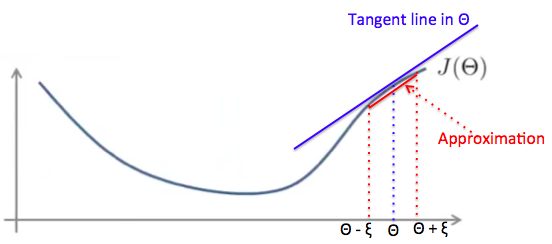
\includegraphics[scale=0.40]{images/gradcheckapprox}
\end{center}
\caption{Gradient checking approximation } 
\label{fig:gradcheckapprox}
\end{figure}

Looking at figure \ref{fig:gradcheckapprox}, the true derivative is the slope of the tangent line in point $\Theta$ (the blue line), but the line that connects the points $(\Theta - \varepsilon, \Theta + \varepsilon)$ (the red line) seem to be a very good approximation. 

Mathematically, the slope of the ``approximation'' line is given by the vertical height $b$, divided by the horizontal width $a$(see figure \ref{fig:approxcomput} ).

\begin{figure}[H]
\begin{center}
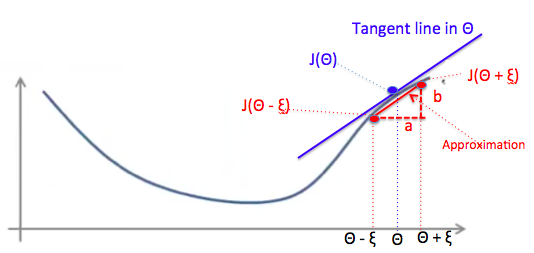
\includegraphics[scale=0.40]{images/approxcomput}
\end{center}
\caption{Gradient checking approximation computation } 
\label{fig:approxcomput}
\end{figure}

Looking at figure \ref{fig:approxcomput} we can define equation \ref{eq:approxcomput}:

\begin{eqfloat}[H]
\begin{equation}
	\begin{aligned}
	a = 2 \varepsilon \\
	b = J(\Theta + \varepsilon) - J(\Theta - \varepsilon)\\
	\frac{\partial}{\partial \Theta} J(\Theta) \approx \frac{J(\Theta + \varepsilon) - J(\Theta - \varepsilon)}{2 \varepsilon}
	\end{aligned}	
\end{equation}
      \addtocounter{equation}{-1}
        \caption{ Gradient checking approximation computation}
        \label{eq:approxcomput}
    \end{eqfloat}

So, $ 	\frac{\partial}{\partial \Theta} J(\Theta) \approx \frac{J(\Theta + \varepsilon) - J(\Theta - \varepsilon)}{2 \varepsilon}
$ is the approximation of the derivative.

Usually $\varepsilon$ is a very small value (like $\varepsilon = 10^{-4}$). If we use a value of $\varepsilon$ excessively small we'll obtain actually the derivative and not the approximation ( looking at figure \ref{fig:approxcomput} we can notice that for values of  $\varepsilon$ excessively small the approximation line -red line- will correspond to the tangent line in $\Theta$-the blue line- so the derivative will be not an approximation but the real value).

In Matlab we will implement the computation of the approximation as follows:


\begin{mdframed}[style=MyFrame]
\begin{lstlisting}
gradApprox = (J(theta + EPSILON) - J(theta - EPSILON) ) / (2 *  EPSILON) 
\end{lstlisting}
\end{mdframed}

\newpage
\begin{mdframed}[style=MyFrame]
\subsubsection{Exercise}
Let $J(\Theta) = \Theta^3$. Furthermore, let $\Theta = 1$ and $\varepsilon = 0,01$. You use the formula 
$\frac{J(\Theta + \varepsilon) - J(\Theta - \varepsilon)}{2 \varepsilon}$
to approximate the derivative. What value do you get using this approximation? (When using $\Theta = 1$ the true exact derivative is $\frac{\partial}{\partial \Theta} J(\Theta) = 3$)

\subsubsection{Solution}
\begin{itemize}
\item $J(\Theta) = \Theta^3$ \\
\item $\Theta = 1$ \\
\item $\varepsilon = 0,01$\\
\item $\Theta + \varepsilon = 1 + 0,01 = 1,01$ \\
\item $\Theta - \varepsilon = 1 - 0,01 = 0,99$ \\
\item $J(\Theta + \varepsilon) = 1,01^3 = 1,030301$\\
\item $J(\Theta - \varepsilon) = 0,99^3 = 0,970299$\\
\item $2 *  \varepsilon = 2 *0,01  = 0,02$\\
\item $\frac{J(\Theta + \varepsilon) - J(\Theta - \varepsilon)}{2 \varepsilon} = \frac{1,030301 - 0,970299}{0,02} = 3,001$
\end{itemize}
\end{mdframed}

Till now we considered the case of $\Theta \in \mathbb{R}$. Now consider the case of where $\Theta$ is a vector parameter, so: \\

\begin{itemize}
\item $\Theta \in \mathbb{R}^n$ (e.g., $\Theta$ is the {\it unrolled} version of $\Theta^{(1)}, \Theta^{(2)}, \Theta^{(3)}$) \\

\item $\Theta = \Theta^{(1)}, \Theta^{(2)}, \Theta^{(3)}$ \\
\end{itemize}
Starting from the approximation just described, for the case of where $\Theta$ is a vector we can use a similar idea to approximate all the partial derivative terms :

\begin{eqfloat}[H]
\begin{equation}
	\begin{aligned}	
	\frac{\partial}{\partial \Theta_1} J(\Theta) \approx \frac{J(\textcolor{red}{\Theta_1 + \varepsilon}, \Theta_2, \Theta_3, \hdots, \Theta_n) - J(\textcolor{red}{\Theta_1 - \varepsilon}, \Theta_2, \Theta_3, \hdots, \Theta_n)}{2 \varepsilon} \\
		\frac{\partial}{\partial \Theta_2} J(\Theta) \approx \frac{J(\Theta_1,\textcolor{red}{ \Theta_2 + \varepsilon} , \Theta_3, \hdots, \Theta_n) - J(\Theta_1,\textcolor{red}{ \Theta_2 - \varepsilon}, \Theta_3, \hdots, \Theta_n)}{2 \varepsilon} \\
\vdots \\
		\frac{\partial}{\partial \Theta_n} J(\Theta) \approx \frac{J(\Theta_1, \Theta_2, \Theta_3, \hdots, \textcolor{red}{\Theta_n+ \varepsilon}) - J(\Theta_1, \Theta_2, \Theta_3, \hdots, \textcolor{red}{\Theta_n - \varepsilon})}{2 \varepsilon} \\
	\end{aligned}	
\end{equation}
      \addtocounter{equation}{-1}
        \caption{ Gradient checking approximation computation, case $\Theta \in \mathbb{R}^n$ }
        \label{eq:approxcomputthetavec}
    \end{eqfloat}
    
Equation \ref{eq:approxcomputthetavec} give us  way to numerically approximate the partial derivative of $J$ with respect to anyone of the parameters. 

Concretely in Matlab we have to implement the following code:

\begin{mdframed}[style=MyFrame]
\begin{lstlisting}
for i=1:n,
	thetaPlus = theta;
	thetaPlus(i) = thetaPlus(i) + EPSILON;
	thetaMinus = theta;
	thetaMinus(i) = thetaMinus(i) - EPSILON;
	gradApprox(i) = (J(thetaPlus) - J(thetaMinus)) / (2 * EPSILON)
end;
\end{lstlisting}
\end{mdframed}

The above code computes the partial derivatives of the cost function (or a good approximation of the derivatives) with respect to every parameter in the neural network; in the ``for'' loop, $n$ is the dimension of the parameter vector $\Theta$. Usually it is better to run that code with the {\it unrolled} version of the parameters. So, $\Theta$ is a long vector of all the parameters in the neural network.

At this point we can compare the derivative numerically computed with the gradient checking $gradApprox$ with the derivatives we obtained with the backpropagation algorithm $DVec$ (remember that the backpropagation is an efficient algorithm to compute the derivatives,or partial derivatives, of the cost function with respect to all of our parameters).

If $gradApprox \approx DVec$ we are more confident that the implementation of the backpropagation algorithm is correct. Summarizing, in the following all steps needed in order to do a correct implementation of the back propagation algorithm are reported:

\begin{itemize}
\item Implement backpropagation to compute {\bf DVec} (unrolled $D^{(1)}, D^{(2)}, D^{(3)}$).
\item Implement numerical gradient checking to compute {\bf gradApprox}.
\item Make sure they give very similar values.
\item Turn off gradient checking and use backpropagation for learning.
\end{itemize}

{\bf Note:} It is very important to disable the gradient checking code before to train the classifier. If we run the numerical gradient computation on every iteration of gradient descent (or in the inner loop of  {\bf costFunction($\hdots$)}) the code will be very slow.



\subsection{Neural networks: Random initialization}

In previous lectures we have seen that for gradient descent and the advance optimization methods we needed some initialization values for $\Theta$:

\begin{mdframed}[style=MyFrame]
\begin{lstlisting}
optTheta = fminunc(@costFunction, initialTheta, options)
\end{lstlisting}
\end{mdframed}

Considering the gradient descent it is possible to initialize $\Theta$ to a vector of zeros (as we did in logistic regression):
\begin{mdframed}[style=MyFrame]
\begin{lstlisting}
initialTheta = zeros(n,1)
\end{lstlisting}
\end{mdframed}

The above initialization works well with the logistic regression, but {\bf it does not work} if we are training a neural network. 

\begin{figure}[H]
\begin{center}
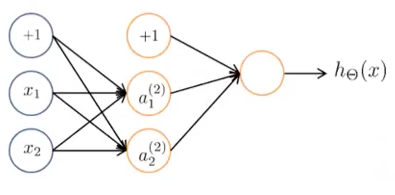
\includegraphics[scale=0.35]{images/nninitialization}
\end{center}
\caption{Neural Network initialization } 
\label{fig:nninitialization}
\end{figure}
 
Consider the neural network in figure \ref{fig:nninitialization}. If we initialize all parameters $\Theta$ to zero, that means that both the hidden unit $a_1^{(2)}$ and $a_2^{(2)}$ are going to compute the same function:



\begin{equation}\label{eq:hid}
\begin{aligned}
a_1^{(2)}  = g(z_1^{(2)}) \implies z_1^{(2)} = \Theta_{10}^{(1)}x_0 + \Theta_{11}^{(1)}x_1 +  \Theta_{12}^{(1)}x_2  = 0\\
a_2^{(2)}  = g(z_2^{(2)}) \implies z_2^{(2)} = \Theta_{20}^{(1)}x_0 + \Theta_{21}^{(1)}x_1 +  \Theta_{22}^{(1)}x_2  = 0\\
a_1^{(2)}  = g(z_1^{(2)}) = g(0) = 0.5\\
a_2^{(2)}  = g(z_2^{(2)}) = g(0) = 0.5\\
\end{aligned}
\end{equation}

Also the computation of the $\delta$ values (in the backpropagation algorithm ) presents the same problem, so  $\delta_1^{(2)} = \delta_2^{(2)}$.

What we can show is that the partial derivatives with respect to the parameters will satisfy the following equation:

\begin{equation}\label{eq:initpartderiv}
\frac{\partial}{\partial \Theta_{01}^{(1)}} J(\Theta) = \frac{\partial}{\partial \Theta_{02}^{(1)}} J(\Theta)
\end{equation}


From equation \ref{eq:initpartderiv} we can infer that, even after a gradient descent update, we will obtain that $\Theta_{01}^{(1)} = \Theta_{02}^{(1)}$, so they will be some non-zero values but they will be equal.

After each update, parameters corresponding to inputs going into each of the hidden units are identical; consequently also the different hidden units will compute the same values that the input. With these parameters the neural network is not able to compute an interesting function.

In order to avoid the just described problem (called {\bf Symmetry Breaking}), we initialize the parameters of a neural network with a {\bf random initialization}; so each value of $\Theta$ will be initialed to a random value between $[-\varepsilon, \varepsilon]$ ($-\varepsilon \le \Theta_{ij}^{(l)} \le \varepsilon$). In the following the Matlab code to make a random initialization of $\Theta$:

\begin{mdframed}[style=MyFrame]
\begin{lstlisting}
Theta1 = rand(10,11) * (2 * INIT_EPSILON) - INIT_EPSILON
Theta2 = rand(1,11) * (2 * INIT_EPSILON) - INIT_EPSILON
\end{lstlisting}
\end{mdframed}
Note that {\it $rand(10,11)$} will create a $10 \times 11$ matrix of random values between $[0,1]$, so a value x ($0 \le x \le 1$) multiplied by $(2\varepsilon)-\varepsilon$ give us a real number between $[-\varepsilon ,\varepsilon ]$ (note: the $\varepsilon$ used in random initialization is {\bf unrelated}  from the $\varepsilon$ used in gradient checking).



\subsection{Putting it together}
In this section we'll see all steps needed to train a neural network. The first step consist of choosing a neural network architecture (the architecture is the connectivity pattern between the neural network neurons).\\
{\bf How do we choose the neural network architecture?}\\
\begin{itemize}
\item {\bf Number of input units}: Dimension of features $x^{(i)}$.
\item {\bf Number of output units}: Number of classes.
\item {\bf Number of hidden layer}: A reasonable default is to use a single hidden layer (it is the most common). If you use more than one hidden layer, a reasonable default is to use the same number of hidden units in every single hidden layer.
\item {\bf Number of hidden units}: usually, the more hidden units, the better. On the other hand, consider that a neural network with a lot of hidden units, can became computationally expensive. Usually the number of hidden units in each layer may be comparable to the dimension of the input features $x$; it is common to choose a number slightly higher than the number of the input features. 
\end{itemize}

Following the above guideline, usually lead to a neural network that works very well.

Now we'll see all steps we need to implement to {\bf train a neural network}:
\begin{enumerate}
\item Randomly {\bf initialize weights}.
\item Implement {\bf forward propagation} to get $h_\Theta(x^{(i)})$ for any $x^{(i)}$.
\item Implement code to compute {\bf cost function} $J(\Theta)$.
\item Implement {\bf backpropagation algorithm} to compute partial derivatives $\frac{\partial}{\partial \Theta_{ij}^{(l)}}J(\Theta)$
\item Use {\bf gradient checking} to compare $\frac{\partial}{\partial \Theta_{ij}^{(l)}}J(\Theta)$ computed using backpropagation with that computed using numerical estimate of gradient of $J(\Theta)$ (gradient checking).
\item {\bf disable gradient checking} code.
\item Use gradient descent or any advanced optimization method with back propagation to try to {\bf minimize $J(\Theta)$} as a function of parameter $\Theta$.
\end{enumerate}

Concretely, to implement the backpropagation algorithm, we use a {\it for} loop over the training examples (there are also other methods but they are more complicated):


\begin{mdframed}[style=MyFrame]
%\begin{lstlisting}
\textcolor{blue}{for 1=1:m}\\
	perform forward propagation and back propagation using example $(x^{(i)}, y^{(i)})$\\
	(get activation $a^{(l)}$ and delta terms $\delta^{(l)}$ for $l=2,\hdots,L$)
%\end{lstlisting}
\end{mdframed}

Within the {\it for} loop we compute the {\bf accumulation term}:
\begin{eqfloat}[H]
\begin{equation}
	\Delta^{(l)} = 	\Delta^{(l)} + 	\delta^{(l+1)} (a^{(l)})^T
\end{equation}
      \addtocounter{equation}{-1}
        \caption{ Accumulation term}
        \label{eq:accumulationterm}
    \end{eqfloat}

Outside the {\it for} loop we compute the {\bf partial derivative terms} $\frac{\partial}{\partial \Theta_{uk}^{(l)}}J(\Theta)$ taking into account the regularization term $\lambda$.

How gradient descent works in a neural network might seem a little bit magical. Let's see figure \ref{fig:graddesc} to try to understand the intuition about what gradient descent for a neural network do.


\begin{figure}[H]
\begin{center}
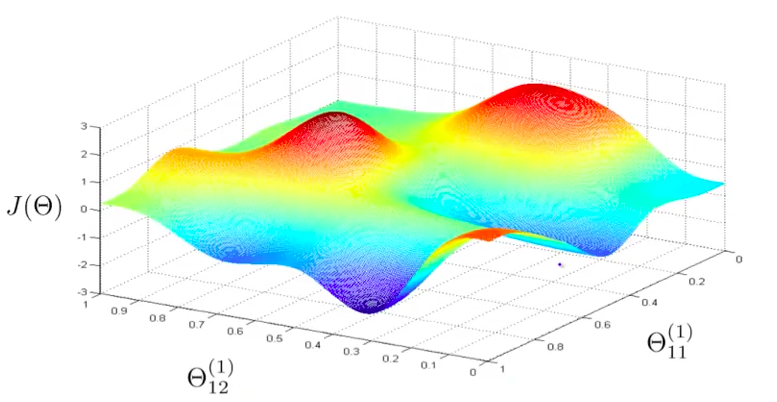
\includegraphics[scale=0.35]{images/graddesc}
\end{center}
\caption{Gradient descent } 
\label{fig:graddesc}
\end{figure}

In figure \ref{fig:graddesc} the cost function $J(\Theta)$ measures how well the neural network fits the training data. The values of $J(\Theta)$ in the figure that are very low corresponds to a setting of the parameters that makes the output $h_\Theta(x^{(i)}) \approx y^{(i)}$.

Gradient descent starts from some random initial points and it repeatedly go down; so, what backpropagation does is to compute the direction of the gradient.
%\input{Chapters/2_RelatedWork}
%\input{Chapters/4_FriendRecommendation.tex}
%\input{Chapters/3_TagRecommendation}
%\input{Chapters/5_SocialMotivation}
%\input{Chapters/6_Conclusions}
%\input{Chapters/8_Appendix_A}


%
% Appentix
%\input{appendices}
%\input{appendicesA.music}
%\input{appendicesB.hci}
%
\cleardoublepage
\phantomsection
\addcontentsline{toc}{part}{References}

%\bibliographystyle{plain}
%\renewcommand{\bibname}{References}
%\bibliography{biblio}



\backmatter
%\input{acknowledgements}

\end{document}
